% Hanning and RFI clipping
%% IEEE stlye bare_jrnl.tex
%% V1.3
%% This is a skeleton file demonstrating the use of IEEEtran.cls
%% (requires IEEEtran.cls version 1.7 or later) with an IEEE journal paper.
%%


% *** Authors should verify (and, if needed, correct) their LaTeX system  ***
% *** with the testflow diagnostic prior to trusting their LaTeX platform ***
% *** with production work. IEEE's font choices can trigger bugs that do  ***
% *** not appear when using other class files.                            ***
% The testflow support page is at:
% http://www.michaelshell.org/tex/testflow/


%%*************************************************************************
%% Legal Notice:
%% This code is offered as-is without any warranty either expressed or
%% implied; without even the implied warranty of MERCHANTABILITY or
%% FITNESS FOR A PARTICULAR PURPOSE! 
%% User assumes all risk.
%% In no event shall IEEE or any contributor to this code be liable for
%% any damages or losses, including, but not limited to, incidental,
%% consequential, or any other damages, resulting from the use or misuse
%% of any information contained here.
%%
%% All comments are the opinions of their respective authors and are not
%% necessarily endorsed by the IEEE.
%%
%% This work is distributed under the LaTeX Project Public License (LPPL)
%% ( http://www.latex-project.org/ ) version 1.3, and may be freely used,
%% distributed and modified. A copy of the LPPL, version 1.3, is included
%% in the base LaTeX documentation of all distributions of LaTeX released
%% 2003/12/01 or later.
%% Retain all contribution notices and credits.
%% ** Modified files should be clearly indicated as such, including  **
%% ** renaming them and changing author support contact information. **
%%
%% File list of work: IEEEtran.cls, IEEEtran_HOWTO.pdf, bare_adv.tex,
%%                    bare_conf.tex, bare_jrnl.tex, bare_jrnl_compsoc.tex
%%*************************************************************************

% Note that the a4paper option is mainly intended so that authors in
% countries using A4 can easily print to A4 and see how their papers will
% look in print - the typesetting of the document will not typically be
% affected with changes in paper size (but the bottom and side margins will).
% Use the testflow package mentioned above to verify correct handling of
% both paper sizes by the user's LaTeX system.
%
% Also note that the "draftcls" or "draftclsnofoot", not "draft", option
% should be used if it is desired that the figures are to be displayed in
% draft mode.
%
%draft \documentclass[11pt,draftcls]{IEEEtran}
\documentclass[journal]{IEEEtran}
% Final \\documentclass[journal]{IEEEtran}
%
% If IEEEtran.cls has not been installed into the LaTeX system files,
% manually specify the path to it like:
% \documentclass[journal]{../sty/IEEEtran}





% Some very useful LaTeX packages include:
% (uncomment the ones you want to load)


% *** MISC UTILITY PACKAGES ***
%
%\usepackage{ifpdf}
% Heiko Oberdiek's ifpdf.sty is very useful if you need conditional
% compilation based on whether the output is pdf or dvi.
% usage:
% \ifpdf
%   % pdf code
% \else
%   % dvi code
% \fi
% The latest version of ifpdf.sty can be obtained from:
% http://www.ctan.org/tex-archive/macros/latex/contrib/oberdiek/
% Also, note that IEEEtran.cls V1.7 and later provides a builtin
% \ifCLASSINFOpdf conditional that works the same way.
% When switching from latex to pdflatex and vice-versa, the compiler may
% have to be run twice to clear warning/error messages.






% *** CITATION PACKAGES ***
%
%\usepackage{cite}
% cite.sty was written by Donald Arseneau
% V1.6 and later of IEEEtran pre-defines the format of the cite.sty package
% \cite{} output to follow that of IEEE. Loading the cite package will
% result in citation numbers being automatically sorted and properly
% "compressed/ranged". e.g., [1], [9], [2], [7], [5], [6] without using
% cite.sty will become [1], [2], [5]--[7], [9] using cite.sty. cite.sty's
% \cite will automatically add leading space, if needed. Use cite.sty's
% noadjust option (cite.sty V3.8 and later) if you want to turn this off.
% cite.sty is already installed on most LaTeX systems. Be sure and use
% version 4.0 (2003-05-27) and later if using hyperref.sty. cite.sty does
% not currently provide for hyperlinked citations.
% The latest version can be obtained at:
% http://www.ctan.org/tex-archive/macros/latex/contrib/cite/
% The documentation is contained in the cite.sty file itself.






% *** GRAPHICS RELATED PACKAGES ***
%
\ifCLASSINFOpdf
  % \usepackage[pdftex]{graphicx}
  % declare the path(s) where your graphic files are
  % \graphicspath{{../pdf/}{../jpeg/}}
  % and their extensions so you won't have to specify these with
  % every instance of \includegraphics
  % \DeclareGraphicsExtensions{.pdf,.jpeg,.png}
\else
  % or other class option (dvipsone, dvipdf, if not using dvips). graphicx
  % will default to the driver specified in the system graphics.cfg if no
  % driver is specified.
  \usepackage[dvips]{graphicx}
  % declare the path(s) where your graphic files are
  % \graphicspath{{../eps/}}
  % and their extensions so you won't have to specify these with
  % every instance of \includegraphics
  % \DeclareGraphicsExtensions{.eps}
\fi
% graphicx was written by David Carlisle and Sebastian Rahtz. It is
% required if you want graphics, photos, etc. graphicx.sty is already
% installed on most LaTeX systems. The latest version and documentation can
% be obtained at: 
% http://www.ctan.org/tex-archive/macros/latex/required/graphics/
% Another good source of documentation is "Using Imported Graphics in
% LaTeX2e" by Keith Reckdahl which can be found as epslatex.ps or
% epslatex.pdf at: http://www.ctan.org/tex-archive/info/
%
% latex, and pdflatex in dvi mode, support graphics in encapsulated
% postscript (.eps) format. pdflatex in pdf mode supports graphics
% in .pdf, .jpeg, .png and .mps (metapost) formats. Users should ensure
% that all non-photo figures use a vector format (.eps, .pdf, .mps) and
% not a bitmapped formats (.jpeg, .png). IEEE frowns on bitmapped formats
% which can result in "jaggedy"/blurry rendering of lines and letters as
% well as large increases in file sizes.
%
% You can find documentation about the pdfTeX application at:
% http://www.tug.org/applications/pdftex





% *** MATH PACKAGES ***
%
%\usepackage[cmex10]{amsmath}
% A popular package from the American Mathematical Society that provides
% many useful and powerful commands for dealing with mathematics. If using
% it, be sure to load this package with the cmex10 option to ensure that
% only type 1 fonts will utilized at all point sizes. Without this option,
% it is possible that some math symbols, particularly those within
% footnotes, will be rendered in bitmap form which will result in a
% document that can not be IEEE Xplore compliant!
%
% Also, note that the amsmath package sets \interdisplaylinepenalty to 10000
% thus preventing page breaks from occurring within multiline equations. Use:
%\interdisplaylinepenalty=2500
% after loading amsmath to restore such page breaks as IEEEtran.cls normally
% does. amsmath.sty is already installed on most LaTeX systems. The latest
% version and documentation can be obtained at:
% http://www.ctan.org/tex-archive/macros/latex/required/amslatex/math/





% *** SPECIALIZED LIST PACKAGES ***
%
%\usepackage{algorithmic}
% algorithmic.sty was written by Peter Williams and Rogerio Brito.
% This package provides an algorithmic environment fo describing algorithms.
% You can use the algorithmic environment in-text or within a figure
% environment to provide for a floating algorithm. Do NOT use the algorithm
% floating environment provided by algorithm.sty (by the same authors) or
% algorithm2e.sty (by Christophe Fiorio) as IEEE does not use dedicated
% algorithm float types and packages that provide these will not provide
% correct IEEE style captions. The latest version and documentation of
% algorithmic.sty can be obtained at:
% http://www.ctan.org/tex-archive/macros/latex/contrib/algorithms/
% There is also a support site at:
% http://algorithms.berlios.de/index.html
% Also of interest may be the (relatively newer and more customizable)
% algorithmicx.sty package by Szasz Janos:
% http://www.ctan.org/tex-archive/macros/latex/contrib/algorithmicx/




% *** ALIGNMENT PACKAGES ***
%
\usepackage{array}
% Frank Mittelbach's and David Carlisle's array.sty patches and improves
% the standard LaTeX2e array and tabular environments to provide better
% appearance and additional user controls. As the default LaTeX2e table
% generation code is lacking to the point of almost being broken with
% respect to the quality of the end results, all users are strongly
% advised to use an enhanced (at the very least that provided by array.sty)
% set of table tools. array.sty is already installed on most systems. The
% latest version and documentation can be obtained at:
% http://www.ctan.org/tex-archive/macros/latex/required/tools/


%\usepackage{mdwmath}
%\usepackage{mdwtab}
% Also highly recommended is Mark Wooding's extremely powerful MDW tools,
% especially mdwmath.sty and mdwtab.sty which are used to format equations
% and tables, respectively. The MDWtools set is already installed on most
% LaTeX systems. The lastest version and documentation is available at:
% http://www.ctan.org/tex-archive/macros/latex/contrib/mdwtools/


% IEEEtran contains the IEEEeqnarray family of commands that can be used to
% generate multiline equations as well as matrices, tables, etc., of high
% quality.


%\usepackage{eqparbox}
% Also of notable interest is Scott Pakin's eqparbox package for creating
% (automatically sized) equal width boxes - aka "natural width parboxes".
% Available at:
% http://www.ctan.org/tex-archive/macros/latex/contrib/eqparbox/





% *** SUBFIGURE PACKAGES ***
%\usepackage[tight,footnotesize]{subfigure}
% subfigure.sty was written by Steven Douglas Cochran. This package makes it
% easy to put subfigures in your figures. e.g., "Figure 1a and 1b". For IEEE
% work, it is a good idea to load it with the tight package option to reduce
% the amount of white space around the subfigures. subfigure.sty is already
% installed on most LaTeX systems. The latest version and documentation can
% be obtained at:
% http://www.ctan.org/tex-archive/obsolete/macros/latex/contrib/subfigure/
% subfigure.sty has been superceeded by subfig.sty.



%\usepackage[caption=false]{caption}
%\usepackage[font=footnotesize]{subfig}
% subfig.sty, also written by Steven Douglas Cochran, is the modern
% replacement for subfigure.sty. However, subfig.sty requires and
% automatically loads Axel Sommerfeldt's caption.sty which will override
% IEEEtran.cls handling of captions and this will result in nonIEEE style
% figure/table captions. To prevent this problem, be sure and preload
% caption.sty with its "caption=false" package option. This is will preserve
% IEEEtran.cls handing of captions. Version 1.3 (2005/06/28) and later 
% (recommended due to many improvements over 1.2) of subfig.sty supports
% the caption=false option directly:
%\usepackage[caption=false,font=footnotesize]{subfig}
%
% The latest version and documentation can be obtained at:
% http://www.ctan.org/tex-archive/macros/latex/contrib/subfig/
% The latest version and documentation of caption.sty can be obtained at:
% http://www.ctan.org/tex-archive/macros/latex/contrib/caption/




% *** FLOAT PACKAGES ***
%
%\usepackage{fixltx2e}
% fixltx2e, the successor to the earlier fix2col.sty, was written by
% Frank Mittelbach and David Carlisle. This package corrects a few problems
% in the LaTeX2e kernel, the most notable of which is that in current
% LaTeX2e releases, the ordering of single and double column floats is not
% guaranteed to be preserved. Thus, an unpatched LaTeX2e can allow a
% single column figure to be placed prior to an earlier double column
% figure. The latest version and documentation can be found at:
% http://www.ctan.org/tex-archive/macros/latex/base/



%\usepackage{stfloats}
% stfloats.sty was written by Sigitas Tolusis. This package gives LaTeX2e
% the ability to do double column floats at the bottom of the page as well
% as the top. (e.g., "\begin{figure*}[!b]" is not normally possible in
% LaTeX2e). It also provides a command:
%\fnbelowfloat
% to enable the placement of footnotes below bottom floats (the standard
% LaTeX2e kernel puts them above bottom floats). This is an invasive package
% which rewrites many portions of the LaTeX2e float routines. It may not work
% with other packages that modify the LaTeX2e float routines. The latest
% version and documentation can be obtained at:
% http://www.ctan.org/tex-archive/macros/latex/contrib/sttools/
% Documentation is contained in the stfloats.sty comments as well as in the
% presfull.pdf file. Do not use the stfloats baselinefloat ability as IEEE
% does not allow \baselineskip to stretch. Authors submitting work to the
% IEEE should note that IEEE rarely uses double column equations and
% that authors should try to avoid such use. Do not be tempted to use the
% cuted.sty or midfloat.sty packages (also by Sigitas Tolusis) as IEEE does
% not format its papers in such ways.


%\ifCLASSOPTIONcaptionsoff
%  \usepackage[nomarkers]{endfloat}
% \let\MYoriglatexcaption\caption
% \renewcommand{\caption}[2][\relax]{\MYoriglatexcaption[#2]{#2}}
%\fi
% endfloat.sty was written by James Darrell McCauley and Jeff Goldberg.
% This package may be useful when used in conjunction with IEEEtran.cls'
% captionsoff option. Some IEEE journals/societies require that submissions
% have lists of figures/tables at the end of the paper and that
% figures/tables without any captions are placed on a page by themselves at
% the end of the document. If needed, the draftcls IEEEtran class option or
% \CLASSINPUTbaselinestretch interface can be used to increase the line
% spacing as well. Be sure and use the nomarkers option of endfloat to
% prevent endfloat from "marking" where the figures would have been placed
% in the text. The two hack lines of code above are a slight modification of
% that suggested by in the endfloat docs (section 8.3.1) to ensure that
% the full captions always appear in the list of figures/tables - even if
% the user used the short optional argument of \caption[]{}.
% IEEE papers do not typically make use of \caption[]'s optional argument,
% so this should not be an issue. A similar trick can be used to disable
% captions of packages such as subfig.sty that lack options to turn off
% the subcaptions:
% For subfig.sty:
% \let\MYorigsubfloat\subfloat
% \renewcommand{\subfloat}[2][\relax]{\MYorigsubfloat[]{#2}}
% For subfigure.sty:
% \let\MYorigsubfigure\subfigure
% \renewcommand{\subfigure}[2][\relax]{\MYorigsubfigure[]{#2}}
% However, the above trick will not work if both optional arguments of
% the \subfloat/subfig command are used. Furthermore, there needs to be a
% description of each subfigure *somewhere* and endfloat does not add
% subfigure captions to its list of figures. Thus, the best approach is to
% avoid the use of subfigure captions (many IEEE journals avoid them anyway)
% and instead reference/explain all the subfigures within the main caption.
% The latest version of endfloat.sty and its documentation can obtained at:
% http://www.ctan.org/tex-archive/macros/latex/contrib/endfloat/
%
% The IEEEtran \ifCLASSOPTIONcaptionsoff conditional can also be used
% later in the document, say, to conditionally put the References on a 
% page by themselves.





% *** PDF, URL AND HYPERLINK PACKAGES ***
%
%\usepackage{url}
% url.sty was written by Donald Arseneau. It provides better support for
% handling and breaking URLs. url.sty is already installed on most LaTeX
% systems. The latest version can be obtained at:
% http://www.ctan.org/tex-archive/macros/latex/contrib/misc/
% Read the url.sty source comments for usage information. Basically,
% \url{my_url_here}.





% *** Do not adjust lengths that control margins, column widths, etc. ***
% *** Do not use packages that alter fonts (such as pslatex).         ***
% There should be no need to do such things with IEEEtran.cls V1.6 and later.
% (Unless specifically asked to do so by the journal or conference you plan
% to submit to, of course. )


% correct bad hyphenation here
\hyphenation{op-tical net-works semi-conduc-tor}


\begin{document}
%
% paper title
% can use linebreaks \\ within to get better formatting as desired
\title{Suppression of Strong Quasi--stationary Narrow--band Signals in Radio
  Interferometry}
%
%
% author names and IEEE memberships
% note positions of commas and nonbreaking spaces ( ~ ) LaTeX will not break
% a structure at a ~ so this keeps an author's name from being broken across
% two lines.
% use \thanks{} to gain access to the first footnote area
% a separate \thanks must be used for each paragraph as LaTeX2e's \thanks
% was not built to handle multiple paragraphs
%

%\author{Michael~Shell,~\IEEEmembership{Member,~IEEE,}
%        John~Doe,~\IEEEmembership{Fellow,~OSA,}
%        and~Jane~Doe,~\IEEEmembership{Life~Fellow,~IEEE}% <-this % stops a space
%\thanks{M. Shell is with the Department
%of Electrical and Computer Engineering, Georgia Institute of Technology, Atlanta,
%GA, 30332 USA e-mail: (see http://www.michaelshell.org/contact.html).}% <-this % stops a space
%\thanks{J. Doe and J. Doe are with Anonymous University.}% <-this % stops a space
%\thanks{Manuscript received April 19, 2005; revised January 11, 2007.}}

\author{W.~D.~Cotton, January 15, 2011%\today% <-this % stops a space
\thanks{National Radio Astronomy Observatory, 520 Edgemont Rd.,
Charlottesville, VA, 22903 USA email: bcotton@nrao.edu}% <-this % stops a space
\thanks{Manuscript received ; revised }}

% note the % following the last \IEEEmembership and also \thanks - 
% these prevent an unwanted space from occurring between the last author name
% and the end of the author line. i.e., if you had this:
% 
% \author{....lastname \thanks{...} \thanks{...} }
%                     ^------------^------------^----Do not want these spaces!
%
% a space would be appended to the last name and could cause every name on that
% line to be shifted left slightly. This is one of those "LaTeX things". For
% instance, "\textbf{A} \textbf{B}" will typeset as "A B" not "AB". To get
% "AB" then you have to do: "\textbf{A}\textbf{B}"
% \thanks is no different in this regard, so shield the last } of each \thanks
% that ends a line with a % and do not let a space in before the next \thanks.
% Spaces after \IEEEmembership other than the last one are OK (and needed) as
% you are supposed to have spaces between the names. For what it is worth,
% this is a minor point as most people would not even notice if the said evil
% space somehow managed to creep in.



% The paper headers
\markboth{Obit Development Memo Series No. 23}%
{Shell \MakeLowercase{\textit{et al.}}: Hanning and Strong RFI}
% The only time the second header will appear is for the odd numbered pages
% after the title page when using the twoside option.
% 
% *** Note that you probably will NOT want to include the author's ***
% *** name in the headers of peer review papers.                   ***
% You can use \ifCLASSOPTIONpeerreview for conditional compilation here if
% you desire.




% If you want to put a publisher's ID mark on the page you can do it like
% this:
%\IEEEpubid{0000--0000/00\$00.00~\copyright~2007 IEEE}
% Remember, if you use this you must call \IEEEpubidadjcol in the second
% column for its text to clear the IEEEpubid mark.



% use for special paper notices
%\IEEEspecialpapernotice{(Invited Paper)}




% make the title area
\maketitle


\begin{abstract}
%\boldmath
A discussion is given of the effects of strong, quasi--stationary
narrow band interfering signals on radio interferometry data.
Some techniques for dealing with such signals are described and
examples given.
\end{abstract}
% IEEEtran.cls defaults to using nonbold math in the Abstract.
% This preserves the distinction between vectors and scalars. However,
% if the journal you are submitting to favors bold math in the abstract,
% then you can use LaTeX's standard command \boldmath at the very start
% of the abstract to achieve this. Many IEEE journals frown on math
% in the abstract anyway.

% Note that keywords are not normally used for peerreview papers.
\begin{IEEEkeywords}
Radio Interferometry, RFI flagging
\end{IEEEkeywords}


\section{Introduction}
% The very first letter is a 2 line initial drop letter followed
% by the rest of the first word in caps.
% 
% form to use if the first word consists of a single letter:
% \IEEEPARstart{A}{demo} file is ....
% 
% form to use if you need the single drop letter followed by
% normal text (unknown if ever used by IEEE):
% \IEEEPARstart{A}{}demo file is ....
% 
% Some journals put the first two words in caps:
% \IEEEPARstart{T}{his demo} file is ....
% 
% Here we have the typical use of a "T" for an initial drop letter
% and "HIS" in caps to complete the first word.
% for IEEE journal papers produced under \LaTeX\ using
% IEEEtran.cls version 1.7 and later.
% You must have at least 2 lines in the paragraph with the drop letter
% (should never be an issue)
\IEEEPARstart{I}{mprovements} in sensitivity resulting from the very
wide bandwidths of radio interferometers such as the EVLA come at the
cost of being sensitive to the many terrestrial radio signals which
are many orders of magnitude stronger that the celestial signals of
interest. 
These signals appear in a variety of forms; signals from low earth
orbit satellites appear only for limited periods of time while
those from fixed transmitters such as microwave links are persistent.
These signals may be continuous or impulsive in either time or frequency

Many of these signals are sufficiently strong that they can serious
corrupt calibration of the data as well as any images derived from
them. 
This memo describes some of the effects of strong, quasi--stationary
narrow band signals in the interferometer passband and details some
techniques for dealing with them.
An example is given using  EVLA C band data.
In the following, these strong signals will be referred to as
``interference'' or ``RFI'' in spite of the fact that most are
completely legitimate transmissions.
The techniques discussed are implemented in the Obit package
(\cite{OBIT}, 
http://www.cv.nrao.edu/$\sim$bcotton/Obit.html).

\section{RFI and Radio Interferometers}
% Raw data
\begin{figure}
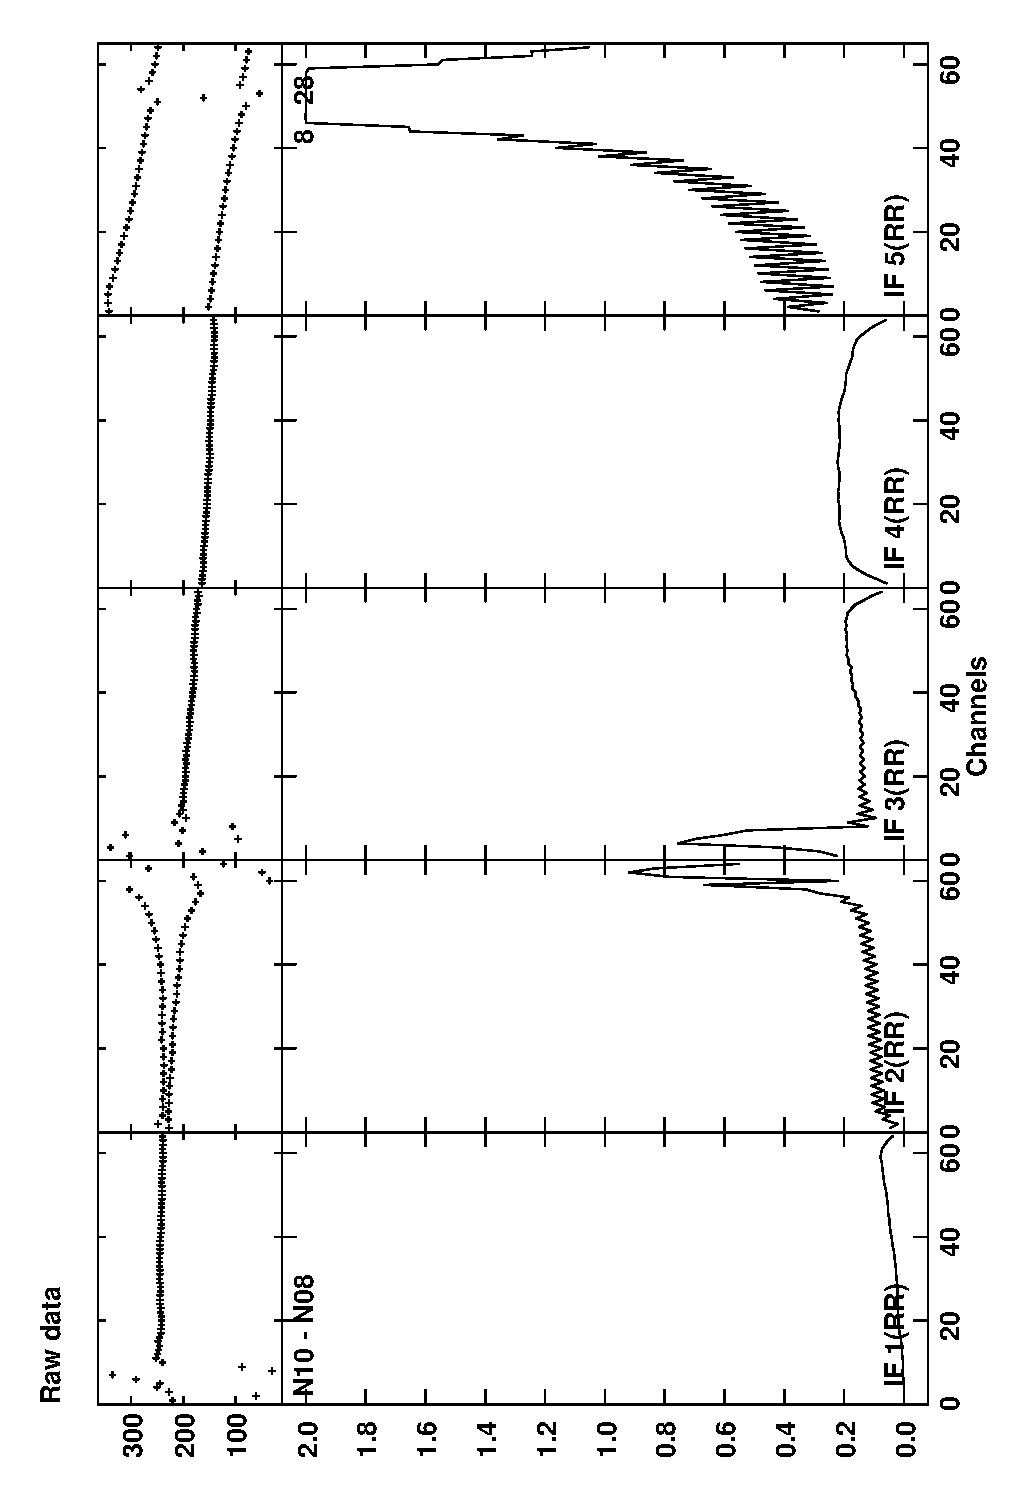
\includegraphics[angle=-90,width=3.5in]{figs/noHann.eps}
\caption{ 
Raw data on 3C286 on one baseline from 6.00 to 6.64 GHz.
The strong interference causes ringing over wide frequency ranges.
The upper plots are the phases in degrees and the lower plots are
amplitudes clipped at 2.0.
} 
\label{RawFig}
\end{figure}

Modern wide-band interferometers record data in multiple sub-bands of
the total bandpass and each of these sub-bands is divided into multiple
channels.
The spectral resolution within a sub-band is usually provided by some
variation on a Fourier transform spectrometer with a limited range of
lags (AKA delays) measured.
Strong, narrow band signals will have significant power at lags not
measured.
The truncation of the lag spectrum may result in ringing of the
response in frequency.
An example of this is shown in Figure \ref{RawFig}.
This figure illustrates the effects of strong signals appearing in
several sub-bands of data on a strong calibrator.
The ringing appears as oscillations in both amplitude and phase as is
strongly seen in the fifth sub-band.
Uncorrected, this ringing can render all data for a given sub-band
useless.

\subsection{Hanning Smoothing}
% Hanned data
\begin{figure}
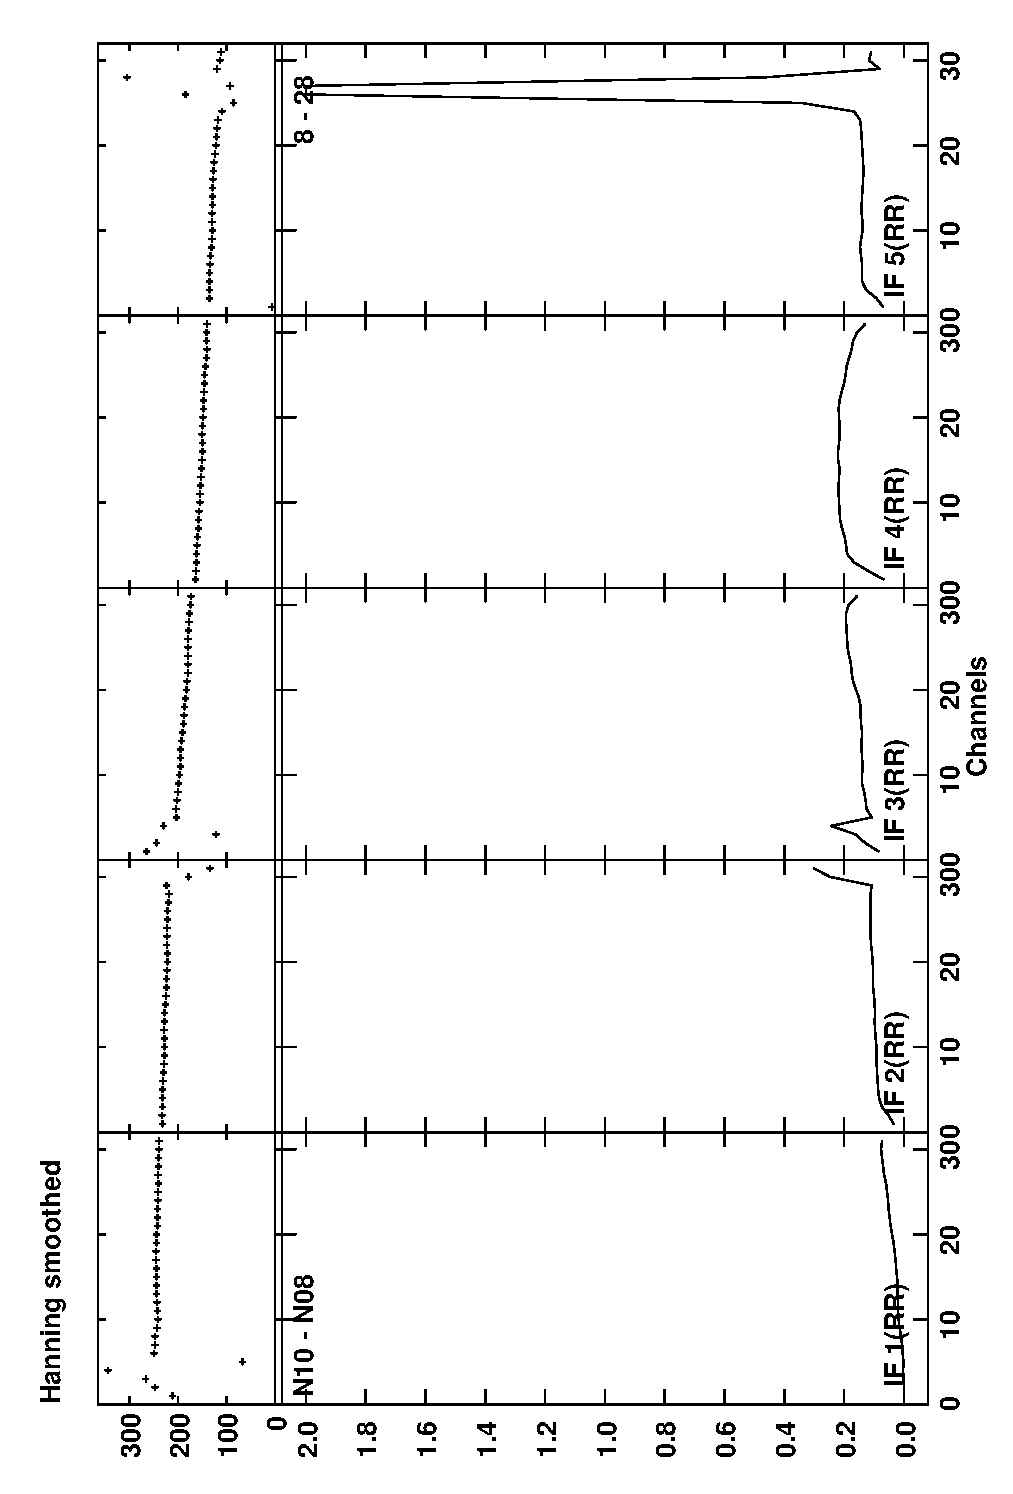
\includegraphics[angle=-90,width=3.5in]{figs/HannSmo.eps}
\caption{ 
Like Figure \ref{RawFig} but after applying Hanning smoothing.
} 
\label{HannFig}
\end{figure}

The traditional solution to this ringing is Hanning smoothing of the
spectrum.
This is a simple convolution of the spectrum with a triangle function
of weights 0.25, 0.5 and 0.25 which effectively cuts the spectral
resolution in half.
Only every other channel is kept after Hanning smoothing.
The data shown in Figure  \ref{RawFig} was Hanning smoothed using Obit
task Hann and the results are given in Figure \ref{HannFig}.
The Hanning has very effectively suppressed the ringing leaving only
the channels directly affected by the signals corrupted.

\subsection{RFI Removal Strategy}
If the interfering signal is sufficiently strong that either the gain
of the amplifier is depressed or there are insufficient bits in the
A/D conversion to represent the celestial signals in the presence of
RFI, the data are irreparably corrupted and should be discarded
While Hanning limits the effects of strong but less damaging signals
to the channels corresponding to the frequencies of the emission,
these channels should be ignored in subsequent processing, an action
referred to as ``flagging''.

% Hann+RFI 
\begin{figure}
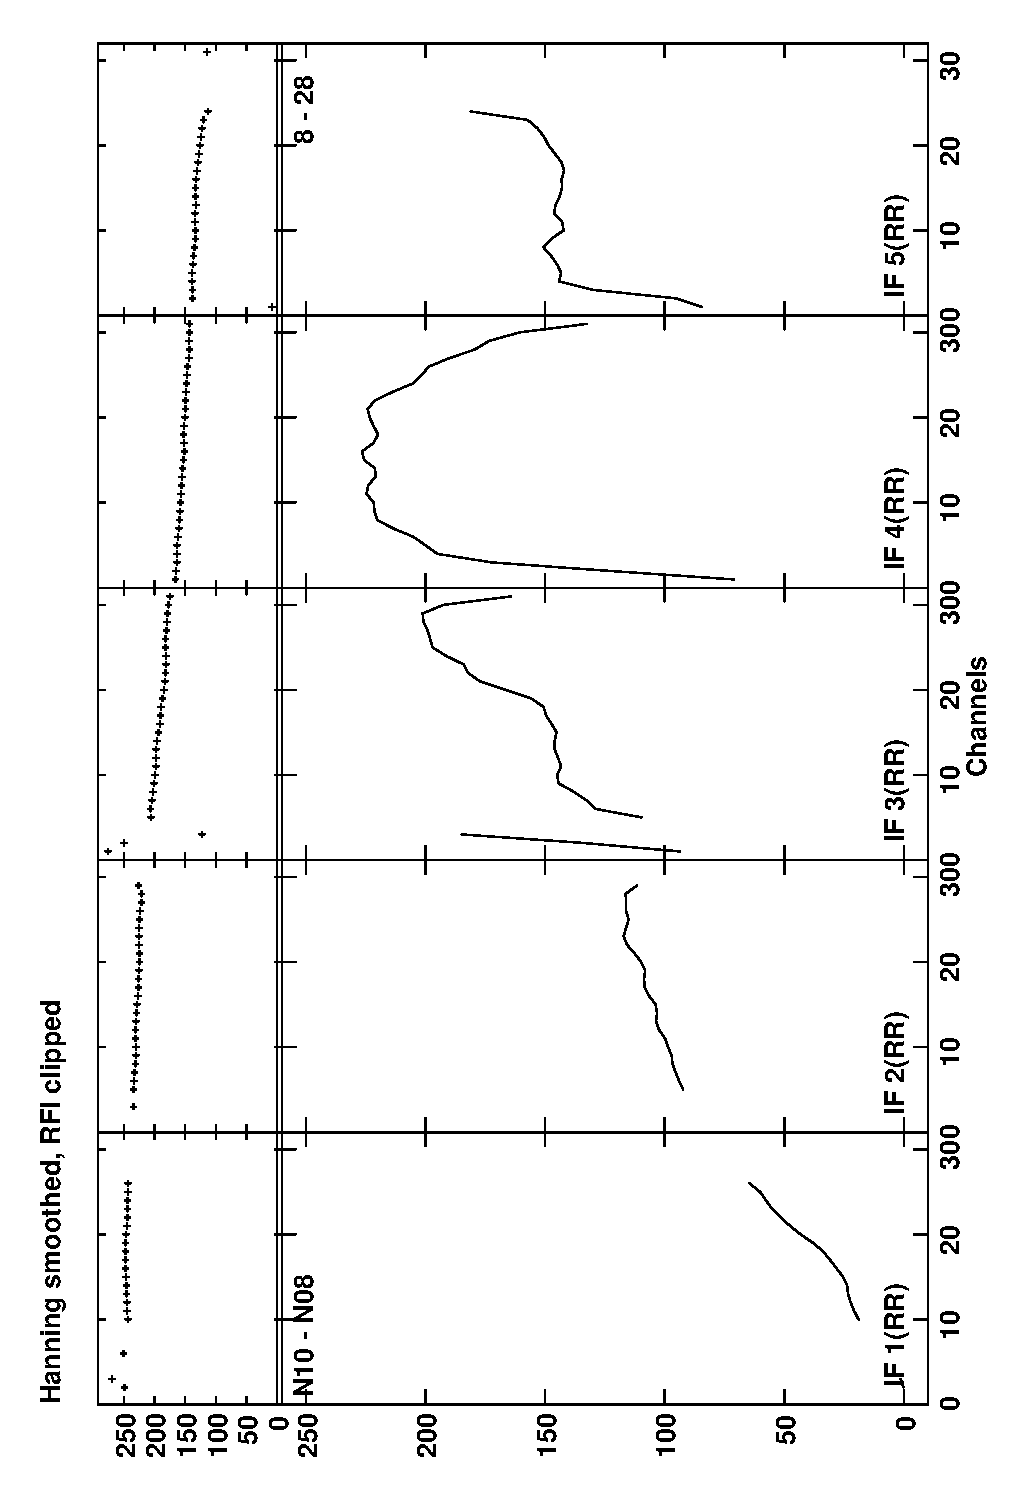
\includegraphics[angle=-90,width=3.5in]{figs/HannRFI.eps}
\caption{ 
Like Figure \ref{HannFig} but after flagging channels differing from a
median.
Note change of scale.
} 
\label{HannRFIFig}
\end{figure}

% Hann+RFI+bandpass
\begin{figure}
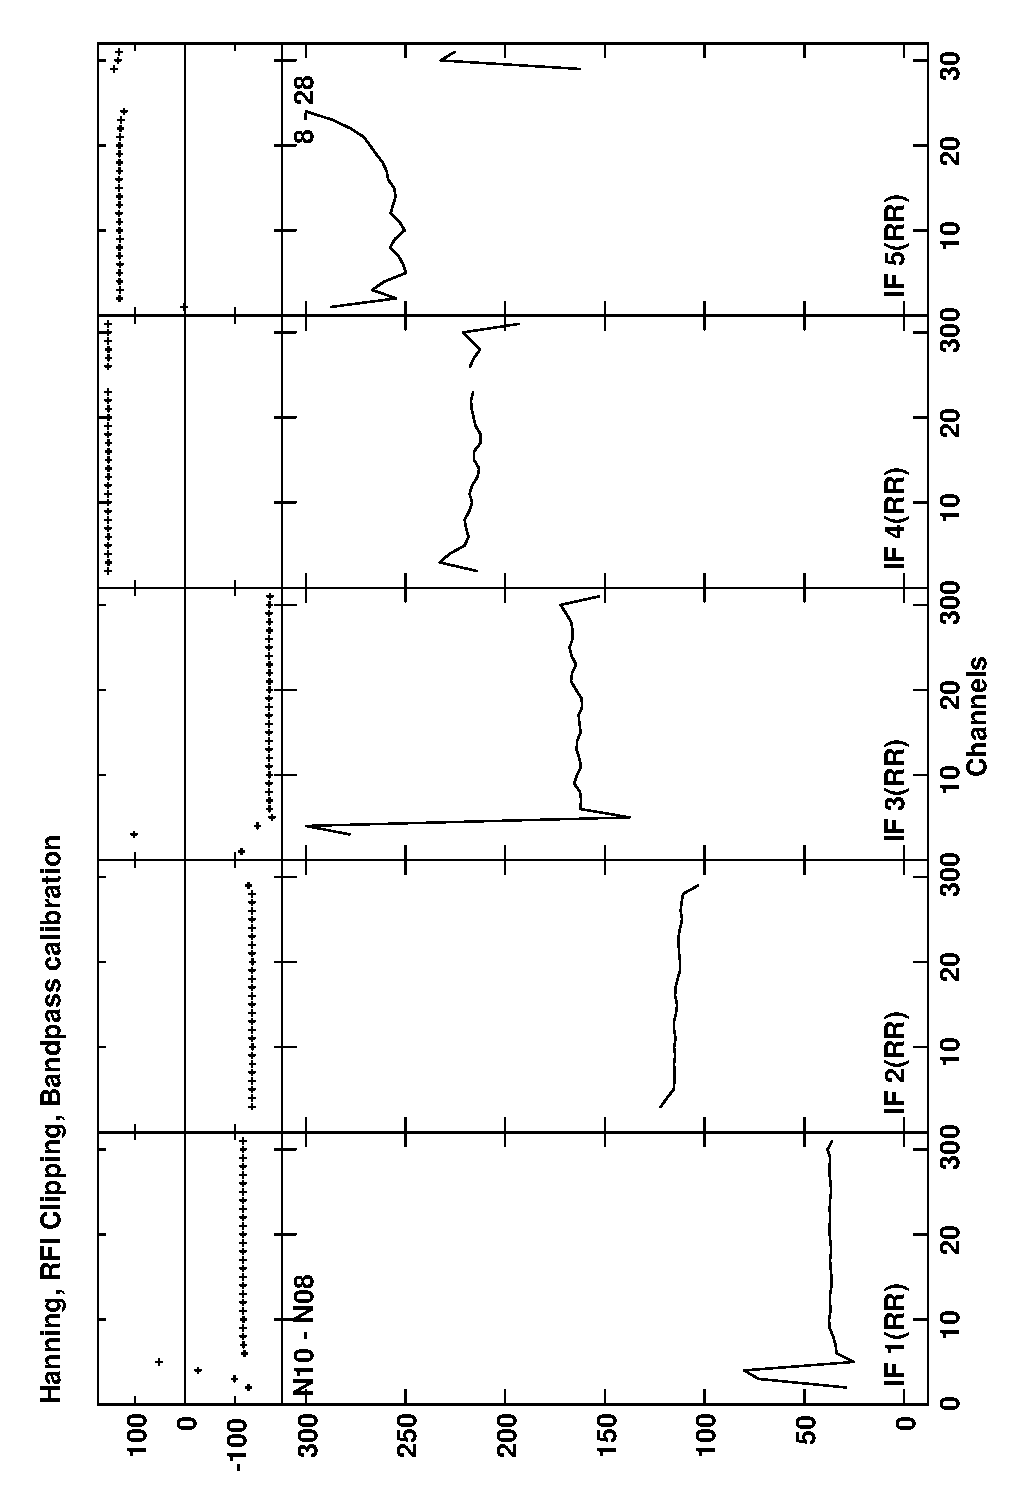
\includegraphics[angle=-90,width=3.5in]{figs/HannRFIBP.eps}
\caption{ 
Like Figure \ref{HannRFIFig} but after bandpass calibration.
} 
\label{HannRFIBPFig}
\end{figure}

% Hann+RFI+bandpass+RFI
\begin{figure}
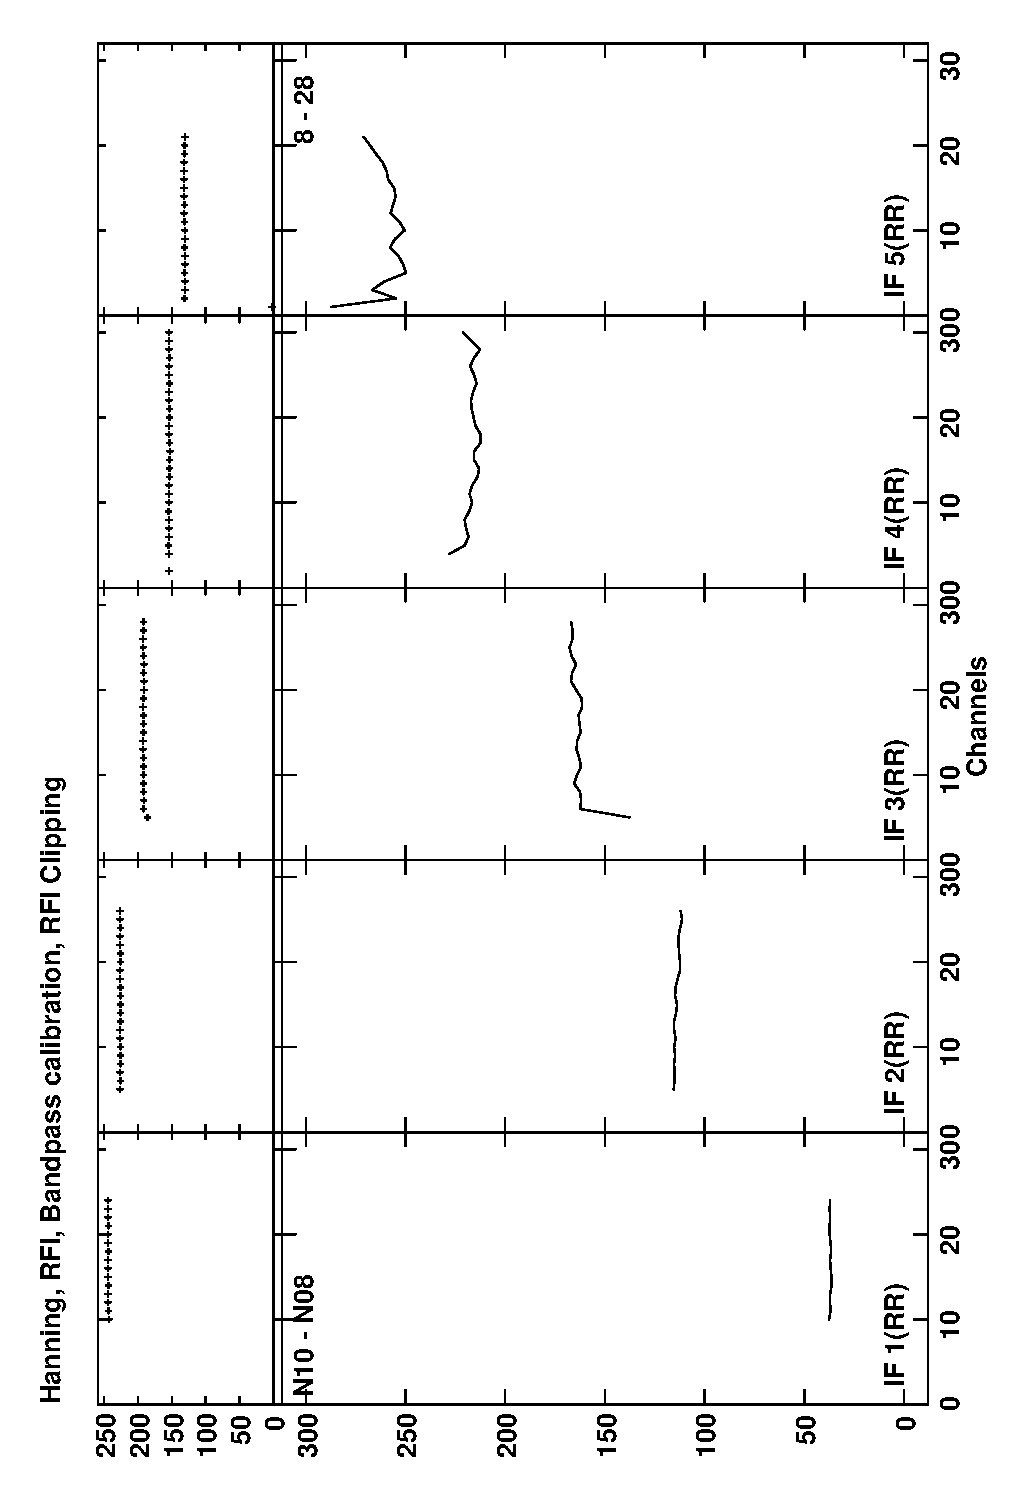
\includegraphics[angle=-90,width=3.5in]{figs/HannRFIBPRFI.eps}
\caption{ 
Like Figure \ref{HannRFIBPFig} but after another RFI flagging.
} 
\label{HannRFIBPRFIFig}
\end{figure}

Assuming the data not to be completely and irreparably corrupted, the
following procedure appears to result in limiting the effects of
strong narrow band interference and eliminating the directly affected
channels; details are given below,
\begin{enumerate}
\item {\bf Hanning Smooth}
As shown above, Hanning very effectively removes the ringing resulting
from the truncated lag spectrum.
The effects of Hanning are the differences between Figures \ref{RawFig} and
\ref{HannFig}. 
\item {\bf Frequency Domain Flagging}
As can be seen in Figure \ref{HannFig}, Hanning smoothed data may contain
RFI contaminated channels which stick out from the unaffected
channels.
These channels can be identified by their contrast with a running
median, assumed to be free of the effects of RFI.
Note, there is a significant channel to channel variation simply due
to the spectral response of the electronics.
This will mask weaker interfering signals.
The results of frequency domain flagging is illustrated in Figure
\ref{HannRFIFig}. 
\item {\bf Bandpass Calibration}
The variation of the gain of the electronics is corrected by a process
known as bandpass calibration in which the instrumental response to a
bright calibrator source is used to determine corrections.
As the interfering signals may be transient, the channels containing
stronger interfering signals should be flagged prior to this calibration.
\item {\bf Deeper Frequency Domain Flagging}
Once the instrumental spectral response has been corrected, a
subsequent frequency domain search for interference can detect and
remove weaker interfering signals.
\end{enumerate}
This procedure should at least be adequate to allow calibration of the
data.
Weaker interfering signals may still be present which adversely affect
the derived images;  these interferences must be dealt with by other
means. 

\subsection{Frequency Domain RFI Flagging}
Narrow band signals are by definition impulsive in frequency hence
relatively easy to identify in a frequency domain analysis if
sufficiently strong to appear above the noise.
The technique applied here is to do limited time averaging of the
data and compare each channel with a running median in frequency.
If the channel amplitude deviates from the median by more than a
specified multiple of the estimate of the noise, that channel and
polarization is flagged.
The noise estimate is the root mean square of the least 80\% deviant of
the samples in the median window.
This estimator is relative insensitive to a small number of RFI
affected channels but underestimates the true noise in the absence of
interference.

This process does not depend on prior calibration of the data but
before bandpass calibration, any variation in the channel--to--channel
instrumental gain will be included in the estimate of the noise.
The data shown in Figures \ref{HannRFIFig} and \ref{HannRFIBPRFIFig}
were flagged using Obit task AutoFlag using a 31 channel median (all
channels after Hanning), 2 minute averaging and clipping at 5 times the
estimated noise.
Each sub-band (labeled ``IF'' in the figures) was processed
independently. 

Two passes of frequency domain flagging were used, before and after
bandpass calibration.
The flagging prior to bandpass calibration removed the most discrepant
interference to minimize the corruption of the bandpass calibration.
After bandpass calibration it is easier to distinguish interference
as the variations in instrumental gain have been removed.

\subsection{Bandpass Calibration}
The purpose of bandpass calibration is to remove the
channel--to-channel instrumental variations in gain and phase using
measurements of a strong calibrator.
These are dominated by the sub-band filter response and the phase slope
resulting from residual group delay errors from the correlation.
The spectral index of the calibrator source is included in the
calibration so that variations in calibrator brightness with frequency
are accounted for.

The data shown in Figure \ref{HannRFIBPFig} were calibrated using Obit
task BPass.
BPass first removes temporal variations in phase using a limited set
of channels in a self calibration.
The data are then time averaged and a subsequent self calibration on a
running block of channels is used to derive the bandpass function.
Multiple scans on the bandpass calibrator may be used for either an
average bandpass function or a time variable bandpass correction.

\section{Discussion}
The technique presented of Hanning visibility data affected by strong
narrow band interference greatly suppresses the ringing resulting from
truncation of the visibility lag function.
The remaining interference can be greatly reduced using a combination
of frequency domain flagging and bandpass calibration.
This process will result in data that can be used for an accurate
calibration although lower level interference may still adversely
affect images produced.

Sample EVLA data seriously affected by RFI was shown to be largely
corrected and the RFI affected channel data removed by the suggested
procedure.
Note, data with interference which is impulsive in time can be
identified and flagged using a time domain analysis similar to the
frequency domain analysis described above.
This process was not beneficial to the data presented here but is
available in Obit task MednFlag.

% use section* for acknowledgement
%*\section*{Acknowledgment}
% Can use something like this to put references on a page
% by themselves when using endfloat and the captionsoff option.
\ifCLASSOPTIONcaptionsoff
  \newpage
\fi


% references section

% can use a bibliography generated by BibTeX as a .bbl file
% BibTeX documentation can be easily obtained at:
% http://www.ctan.org/tex-archive/biblio/bibtex/contrib/doc/
% The IEEEtran BibTeX style support page is at:
% http://www.michaelshell.org/tex/ieeetran/bibtex/
\bibliographystyle{IEEEtran}
% argument is your BibTeX string definitions and bibliography database(s)
\bibliography{HannRFI}
%
% insert where needed to balance the two columns on the last page with
% biographies
%\newpage

% You can push biographies down or up by placing
% a \vfill before or after them. The appropriate
% use of \vfill depends on what kind of text is
% on the last page and whether or not the columns
% are being equalized.

%\vfill

% Can be used to pull up biographies so that the bottom of the last one
% is flush with the other column.
%\enlargethispage{-5in}


% that's all folks
\end{document}


\section{Padding}
LaTeX screws up if there are too many floats for a given amount of
text so let's just add some blather and let it include the figures.

LaTeX screws up if there are too many floats for a given amount of
text so let's just add some blather and let it include the figures.

LaTeX screws up if there are too many floats for a given amount of
text so let's just add some blather and let it include the figures.

LaTeX screws up if there are too many floats for a given amount of
text so let's just add some blather and let it include the figures.

% 3C279
\begin{figure}
\centering
\includegraphics[height=3.5in]{figs/3C279BeamGray.ps}
\caption{ 
3C279 Beam image.
The core is saturated and the stretch is a square root to better
display the lower levels.
}
\label{3C279Fig}
\end{figure}

% 10'' beam
\begin{figure}
\centering
\includegraphics[height=3.5in]{figs/GBTBeamGray.ps}
\caption{ 
GBT beam used with 10'' Gaussian core and the outer portion of the
azimuthally averaged 3C279 image.
The core is saturated and the stretch is a square root to better
display the lower levels.
}
\label{GBTBeamFig}
\end{figure}

\subsection {M87}
% M87 Point Spectra
\begin{figure*}
\centering
\centerline{
\includegraphics[height=3.0in,angle=-90]{figs/M87SpecA.ps}
\includegraphics[height=3.0in,angle=-90]{figs/M87SpecB.ps}
}
\centerline{
\includegraphics[height=3.0in,angle=-90]{figs/M87SpecC.ps}
\includegraphics[height=3.0in,angle=-90]{figs/M87SpecD.ps}
}
\centerline{
\includegraphics[height=3.0in,angle=-90]{figs/M87SpecE.ps}
\includegraphics[height=3.0in,angle=-90]{figs/M87SpecF.ps}
}
\caption{ 
Point spectra of M87 at locations indicated in Figure \ref{M87ContFig}.
Fitted values are shown.
``x'' symbols indicate the measured values and the solid line the
fitted spectrum whose paramters are shown on each plot.
}
\label{M87PtSpectraFig}
\end{figure*}

% M87 Contour
\begin{figure}
\centering
\includegraphics[height=3.in,angle=-90]{figs/M87Cont.ps}
\caption{ 
VLA Image of M87 at 8.4 GHz with indications of locations of point
spectra as letters.
Note the logrithmic contour intervals.
}
\label{M87ContFig}
\end{figure}

% M87 Spectral index
\begin{figure}
\centering
\includegraphics[height=3.0in]{figs/M87SpecIndex.ps}
\caption{ 
M87 spectral index.
Region shown is the same as in Figure \ref{M87ContFig}
The intensity is a function of the flux density, saturated and with a
square root stretch.
Colors range from red (-1.0) to blue(-0.6).
}
\label{M87SIFig}
\end{figure}

% M87 Spectral curvature
\begin{figure}
\centering
\includegraphics[height=3.0in]{figs/M87SpecCurve.ps}
\caption{ 
M87 spectral curvature.
Region shown is the same as in Figure \ref{M87ContFig}
The intensity is a function of the flux density, saturated and with a
square root stretch.
Colors range from red (-0.2) to blue(-0.05). 
}
\label{M87SCFig}
\end{figure}

